\documentclass[english,aspectratio=43]{beamer}

\usetheme{Dresden}

\usepackage{babel}
\usepackage{graphicx}
\usepackage{dsfont}

\graphicspath{{img/}{img2/}}

\beamertemplatenavigationsymbolsempty

\newcommand{\examplewidth}{0.6\textwidth}

\title{Computing Highly Occluded Paths}

\subtitle{Algorithms for Geographic Data}

\author[Group 10]{
	Tim van Dalen (0744839)
	\and
	Bram Kohl (0746107)\\
	\and
	Bart van Wezel (0740608)
}

\institute[TU/e]
{
    WIS\\
	Eindhoven University of Technology
}

\date{March 31, 2015}

\subject{Computing Highly Occluded Paths}

\AtBeginSection[]
{
  \begin{frame}
    \frametitle{Outline}
    \tableofcontents[currentsection]
  \end{frame}
}

\begin{document}

	\begin{frame}
		\titlepage
	\end{frame}

	\begin{frame}
		\frametitle{Outline}
		\tableofcontents
		\note{
			Please do not hesitate to ask questions during this lecture.
			The material we treat will continue to build up, so if any of the earlier stuff isn't clear please just raise your hand.
		}
	\end{frame}

	\section{Occluded paths}
	\begin{frame}{Problem}
	\centering
	\Large
	Given a terrain and some observers, we want to calculate a path that has the least chance of detection

	\note{
		Now that that's in place, let's back up and figure out why we would want this
	}
\end{frame}

\subsection{Motivation}
\begin{frame}{Military}
	Planning troop movements in enemy territory

	\vspace{0.5cm}
	\centering
	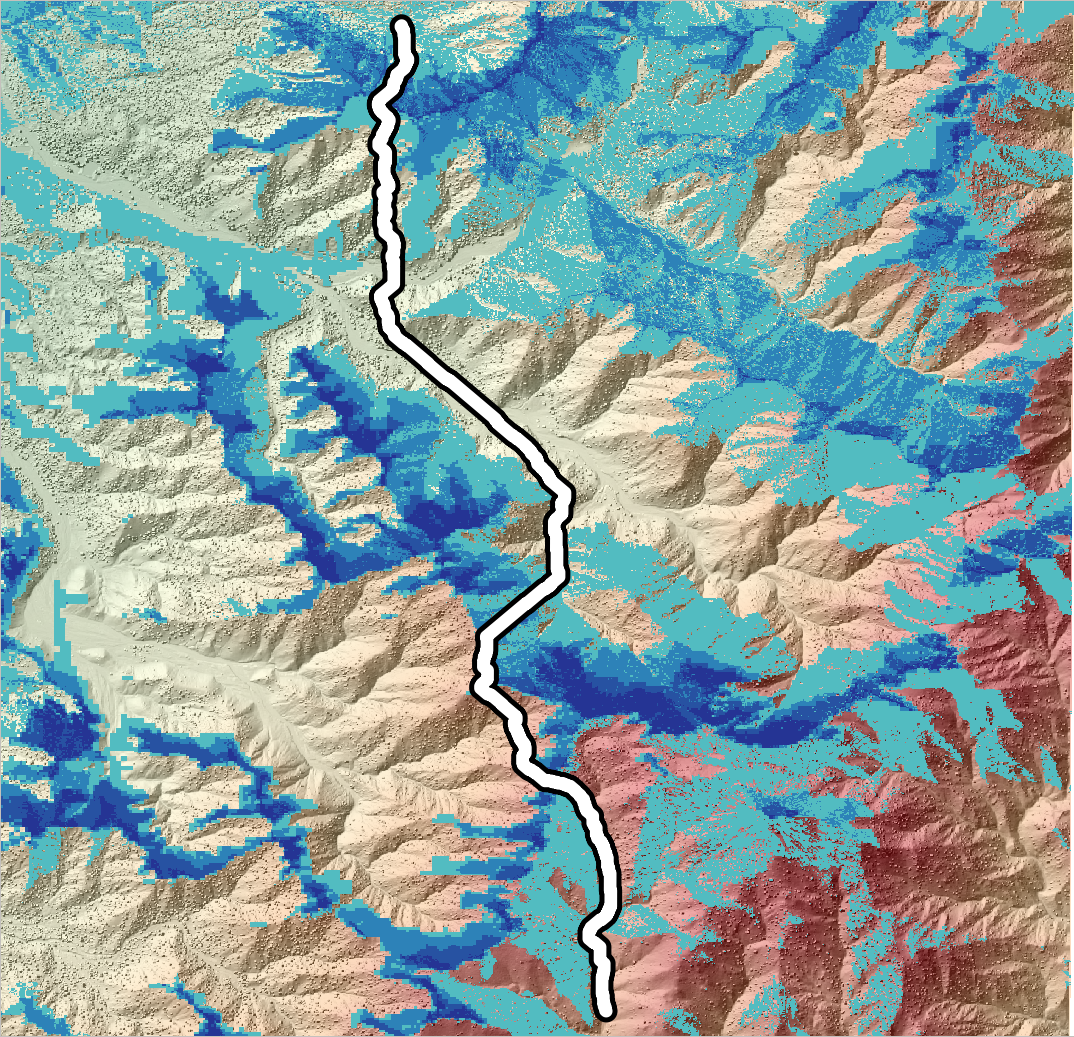
\includegraphics[width=0.35\textwidth]{motivation-military}
\end{frame}

\begin{frame}{City planning}
	Visually unappealing structures

	\vspace{0.5cm}
	\centering
	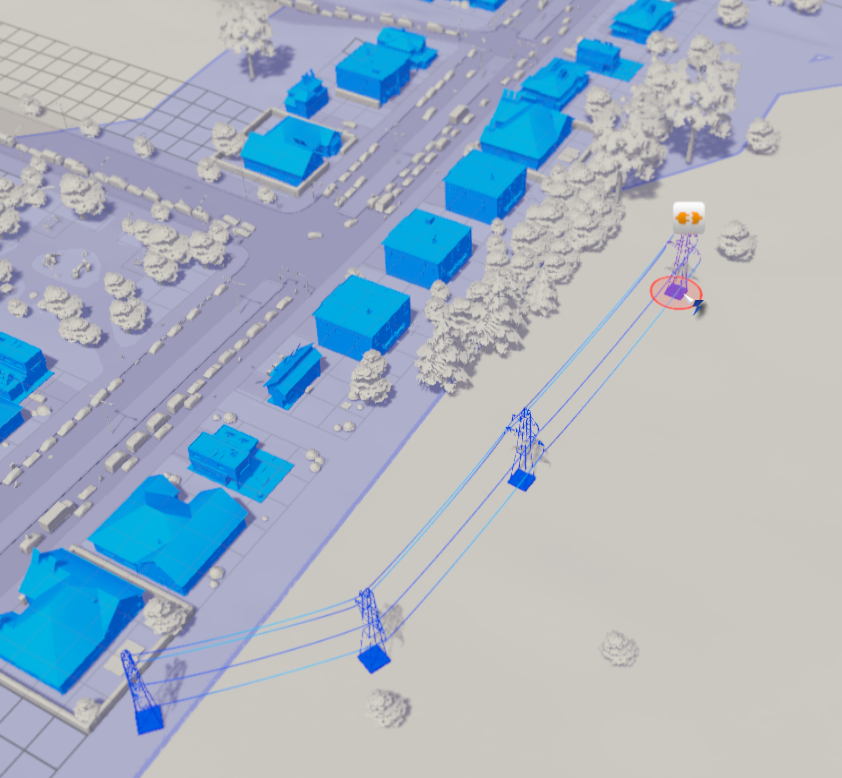
\includegraphics[width=0.35\textwidth]{motivation-city}
\end{frame}

\begin{frame}{Virtual environments}
	Video games

	\vspace{0.5cm}
	\centering
	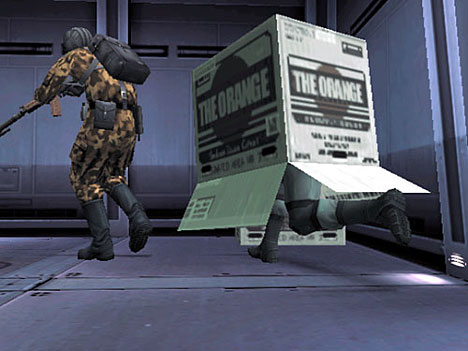
\includegraphics[width=0.45\textwidth]{motivation-virtual}
\end{frame}


\subsection{Terrain}
\begin{frame}{What's a terrain?}
	\begin{itemize}
		\item A map
		\item Elevation
	\end{itemize}

	\note{
		For the rest of the lecture, we'll assume that a terrain is a grid plus a defined height function.
		Note that this representation of terrains can't handle non-convex shapes, so we can't model tunnels or caves using this definition.
	}
\end{frame}

\begin{frame}{Digital Elevation Model}
	\centering
	\only<1>{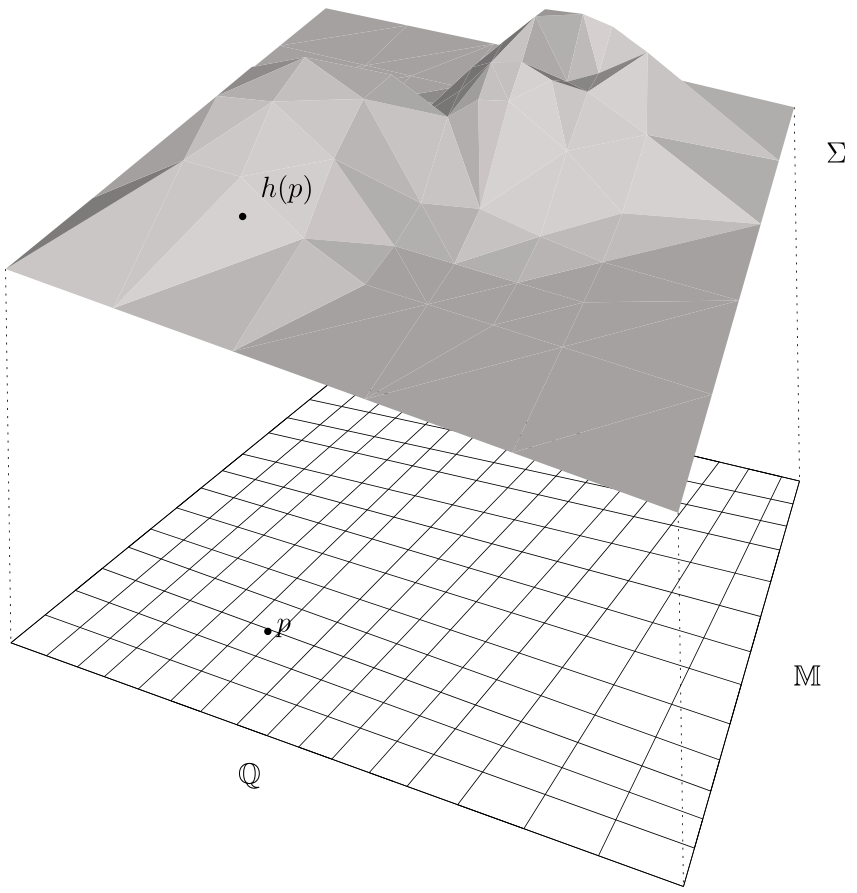
\includegraphics[width=0.6\textwidth]{DEM}}
	\only<2>{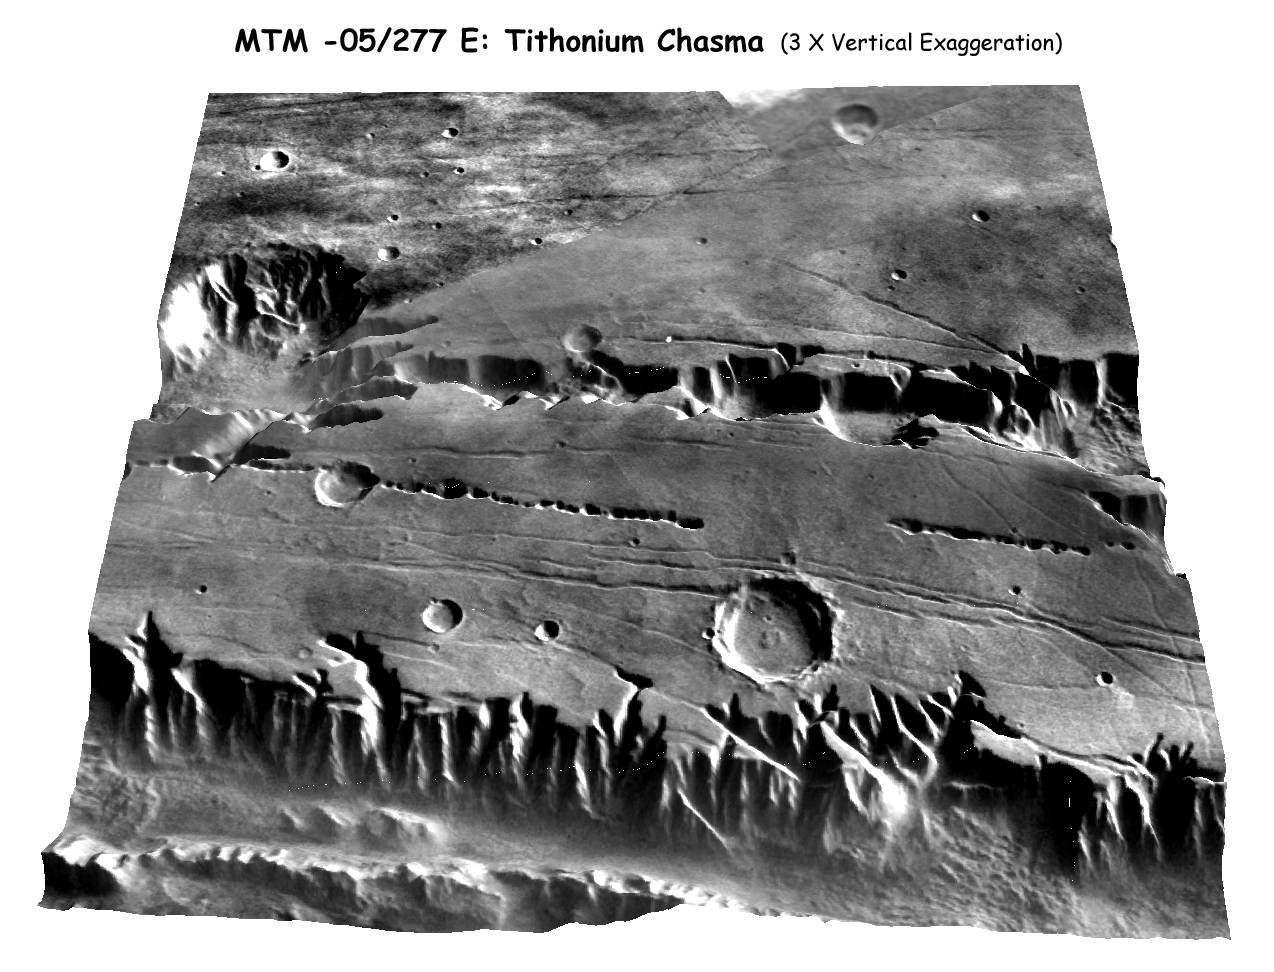
\includegraphics[width=0.8\textwidth]{DEM-mars}}

	\note{
		In particular, we'll be working with DEMs, since they are a common format
	}
\end{frame}

\begin{frame}{Example}
	\centering
	\only<1>{
\includegraphics[width=\examplewidth]{empty}}
	\only<2>{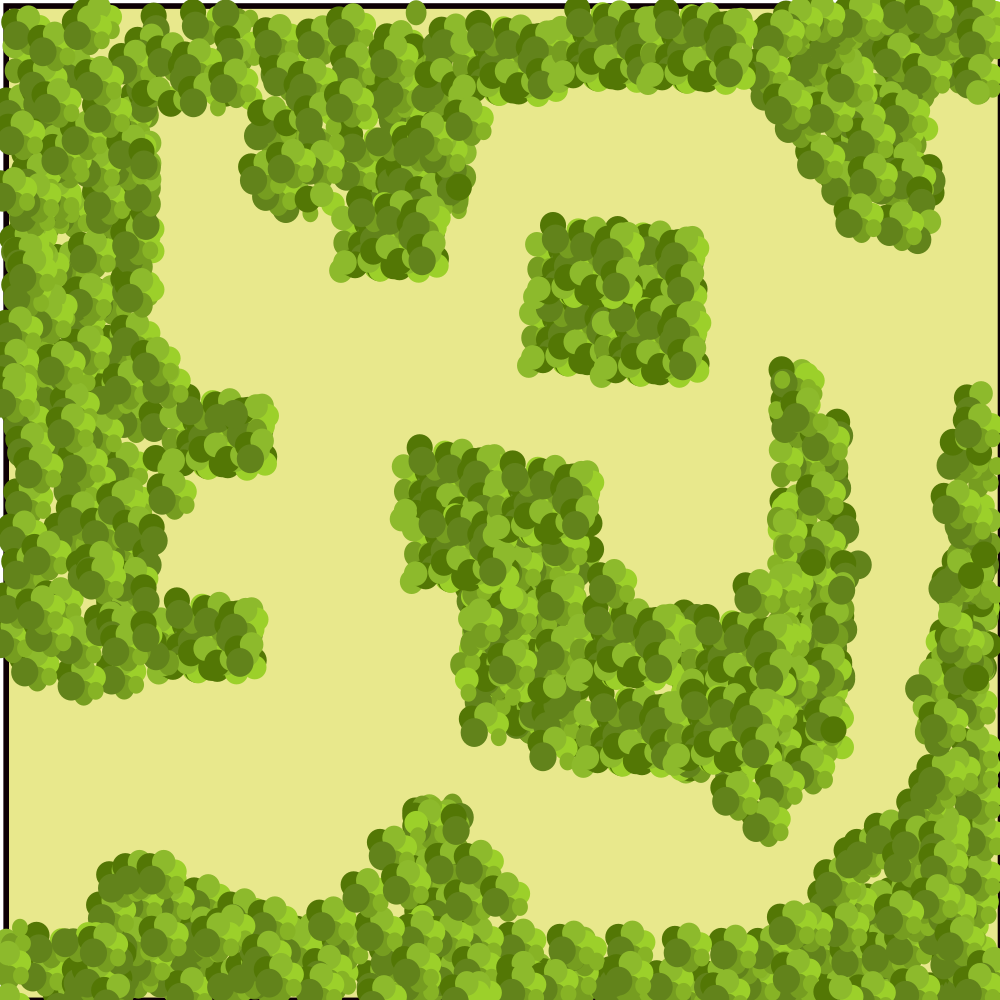
\includegraphics[width=\examplewidth]{terrain}}

	\note{
		Throughout this lecture, we'll work with a very simple example terrain to make it clear what the algorithm is doing.
		We'll start with our grid.

		For elevation, we introduce some trees.
		We do this simply because 3D terrains are hard to get across on slides.
	}
\end{frame}


\subsection{Observers}
\begin{frame}{Observer}
	\begin{itemize}
		\item Entity on the terrain
		\item Visible grid points \note{Those with a clear line of sight}
	\end{itemize}
\end{frame}

\begin{frame}{In our example}
	\centering
	\only<1>{
		\exampleimg{observers}
		\note{So say these dots on the terrain are our observers. We're just going to assume that these are given}
	}%
	\only<2>{
		\exampleimg{observers_visibility}
		\note{
			The next step is to figure out, for each observer, which points on the terrain are visibile and which aren't.
			Of course, the definition of visibilty can be whatever you want it.
			Here, and in the paper we're about to get to, we use that a line from the observer to the point cannot intersect with the height function.
		}
	}%
	\only<3>{
		\exampleimg{observers_line_of_sight}
		\note{However, this isn't realistic as visibily degenerates with distance}
	}%
	\only<4>{
		\exampleimg{observers_line_of_sight_one}
		\note{So we determine, for each observer, how well they can see each point}
	}%
	\only<5>{
		\exampleimg{observers_line_of_sight_all}
		\note{
			And when aggregate that (if we sum the visibility increase from 11 to 12 observers seeing a point would be the same as 1 to 2, so that's not good),
			we end up with the visibility map
		}
	}
\end{frame}


\subsection{Paths}
\begin{frame}{Goal}
	\centering\Large
	Getting from A to B with the lowest chance of detection
	\note{Let's go back to what we actually wanted to achieve here}
\end{frame}

\begin{frame}{Example}
	\centering
	\only<1>{\exampleimg{observers_line_of_sight_all}}%
	\only<2>{\exampleimg{observers_line_of_sight_all_points}}%
	\only<3>{\exampleimg{observers_line_of_sight_all_path}}
\end{frame}




	\section{Algorithm}
	\begin{frame}{Data structures}{Grid DEM}
	\only<1> {
		Recall LiDAR data

		\centering
		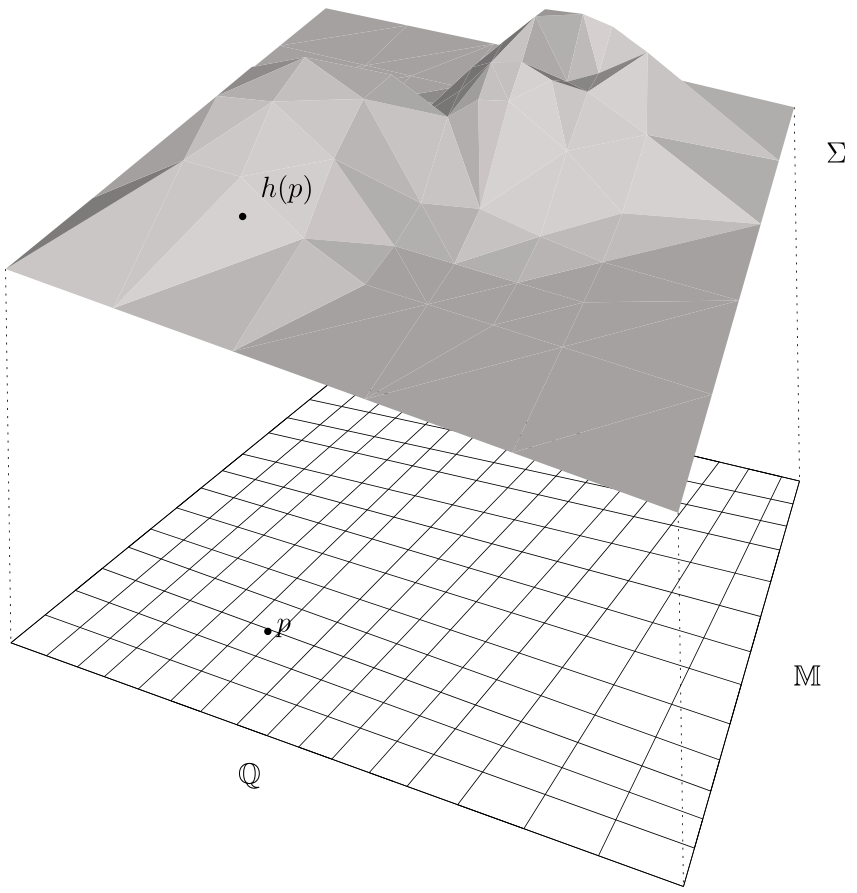
\includegraphics[height=0.5\textheight]{DEM}
	}
	\only<2> {
		We have $\rho > 0, L \geq 0$, $\mathds{M}$ is a square of side length $\rho^{2^L}$, partitioned into $2^L \times 2^L$ grid cells.
	}
\end{frame}

\subsection{Forming the model}
\begin{frame}{Continous}
	\begin{itemize}
		\only<1>{
			\item $\mathds{M}$ is a square region
			\item $h$ is a height function
			\item The graph of $h$, $\Sigma$ is a terrain
		}
		\only<2>{
			%TODO: Illustration
			\item $b$ is visible from $a$ if no point in segment $ba$ lies below $\Sigma$
			\item The visibility map of an observer $o$ is for each point in $\mathds{M}$:\\
				\[V_o(p) = \left\{
					\begin{array}{lr}
						1 & : p \textnormal{ is visible from } o,\\
						0 & : \textnormal{otherwise.}
					\end{array}
					\right.
				\]
			\item Attenuated visibility map
				\note{Takes in account that vision deteriorates}
		}
	\end{itemize}
\end{frame}

\begin{frame}{Observers}
	Given $m$ observers, the aggregated visibility map:
	\[
		V_O(p) = \sum_{i=1}^{m}{V_{o_i}(p)}
	\]
\end{frame}

\begin{frame}{Coverage map}
	\only<1> {
		The coverage map of $\Sigma$, for observers $O$:
		\[
			\omega_O(p) = 1 - \epsilon^{-cV_O(p)}
		\]
		with $c > 0$

		\note{
			Now this looks very interesting, but basically all it does is make the increase in
			visibility between 0 and 1 observers bigger than the increase in visibility
			between 10 and 12 observers seeing a point
		}
	}

	\only<2> {
		The cost of a curve $\Pi$ of length $L$ is:
		\[
			c(\Pi) = \int_0^L \omega(\Pi(t)) dt
		\]
		%TODO: Explain why this is using the integral

		Cost of the most occluded path between $a$ and $b$:
		\[
			\inf_\Pi c(\Pi)
		\]
		%TODO: Explain why you can't just use min...
	}
\end{frame}


\subsection{Computing the visibility map}
\begin{frame}{Simplification}

\end{frame}

\begin{frame}{Computing the map}

\end{frame}

\begin{frame}{Using the GPU}
	\begin{itemize}
		\item GPU is useful for doing many simple calculations
		\item Reformulate visibility map as typical GPU problem
		\item Color pixels based on visbility
		\item Read out color buffer
	\end{itemize}
\end{frame}


\subsection{Computing occluded paths}
\begin{frame}{Known observer placement}
	\begin{itemize}
		\item Compute the visibility map
		\item Compute the coverage map
		\item Construct weighted graph of grid connections
		\item Find minimum-cost path  using Dijkstra
	\end{itemize}
\end{frame}

\begin{frame}{Unknown observer placement}
	\begin{itemize}
		\item Problem becomes finding a good guess for O
		\item Assuming a rational opponent
		\item Assuming a budget of $k$ observers
	\end{itemize}
\end{frame}

\begin{frame}{Unknown observer placement}{Strategies}
	\begin{itemize}
		\only<1>{
			\item Topology-based placement
				\begin{itemize}
					\item Find local maxima in the map
					\item Use contours to find maxima on different hills
					\item Place observers there
				\end{itemize}
		}
		\only<2>{
			\item Coverage-based placement
				\begin{itemize}
					\item Compute visibility map
					\item Place observers to cover as much terrain as possible
				\end{itemize}
		}
	\end{itemize}
\end{frame}



	\section{Networks}
	\begin{frame}{So far...}
	\centering\Large
	We now have a scalable algorithm for computing occluded paths, but what if we are interested in a terrain more than once?
	\pause

	Precomputing!
	\pause

	\begin{thebibliography}{10}
		\beamertemplatearticlebibitems
		\bibitem{agarwal13}
			Niel~Lebeck, Thomas~M\-olhave, Pankaj~K.~Agarwal
		\newblock {\em Computing Highly Occluded Paths Using a Sparse Network}.
		\newblock SIGSPATIAL'14
	\end{thebibliography}

	\note{So now we have found a scalable algorithm for computing occluded paths. 
However finding an occluded path on the visualization map is not really fast.
When we want to compute a lot of occluded paths on a terrain, we can use pre computing.
This is mainly the case with real terrain data and in video games. 
Real terrain data does not change much. Mountains do not move.
In video games the terrain is predefined and does not change at all.
}
\end{frame}

\subsection{Approach}
\begin{frame}{Idea}
	\centering
	\only<1>{\exampleimg{network_ex1}}%
	\only<2>{\exampleimg{network_ex2}}%
	\only<3>{\exampleimg{network_ex3}}
	\note{
		Suppose we have to find some paths between those poinsts. 
		Then we first find this path, then we have to compute this path and finally this path.
		Now you can see that all those paths use the same subpath here. 
		This subpath is now computed three times, which can become very costly if the size of the subpath increases. 
		So the idea is to make a network, so that we only have to compute point A, B to the network.
		After this we can find the lowest weight path between the two points, where A and B connect to the network, to find the path from A to B. 
	}
\end{frame}

\begin{frame}{Approach}
	\begin{itemize}
		\item Compute the visibility map once
		\item Determine a network of occluded paths
		\item Calculate connections to the network
		\item Calculate shortest connection on the network, between the two connected points. 
	\end{itemize}
	note{
		So the approach now will be to compute the visiblity map once. 
		This is so that we can find the best occluded paths on the network, which we want to include. 
		Then we determine a network of the occluded paths that we surely want in the network. 
		When we have a good network, we can easily find a good occluded path between two points. 
		We simply find the best occluded path to the network.
		Then we find the lowest weight connection between the two points on the network. 
	}
\end{frame}



\begin{frame}{Building the network}
	\begin{itemize}
		\item Chosing how to build the network is really important
		\item Well chosen network results in high-quality paths
		\item Paths can become really expensive if the network is not well chosen.
		\item To dense networks result in high computing time for the points on the network where we connect
		\item A network that is to sparse result in high computing time for the connection between the points and the network
	\end{itemize}

	\note{
		Suppose in our example we have a network like this: 
		This would result in occluded paths, that are not really useful. 
		
	}
\end{frame}

\begin{frame}
 	\centering
	\only<1>{\exampleimg{network_fail}}%
	\only<2>{\exampleimg{network_fail2}}%
	\only<3>{\exampleimg{network_fail3}}
\end{frame}

\begin{frame}{Strategies}
	\begin{itemize}
		\item Sampling based
		\item Learning based
		\item Topology based
	\end{itemize}

	\note{
		In the paper they explained multiple ways to build the network. 
		Sampling and learning based are based on the visibility map.
		They compute a lot of occluded paths on the network. 
		Then they look which path are most used and include those paths to the network.
		When the network is not complete yet, they compute the best paths between the subpaths. 
		The difference between sampling and learning based is the following:
		Sampling based takes a number of points on the map. 
		They tried multiple strategies to determine those points. 
		Then they for each of those points they find the occluded paths to his nearest neighbors.
		Learning based also takes a number of points. Here they take random points on the border.
		Then they compute the highest occluded paths to other points on the border. 
		The occluded paths in the learning based strategy are longer and thus takes more time. 
		Topology based is based on the terrain and not on the visibility map.
		Here they try to find local maxima on the terrain and include these points in to the network. 
		Next, we'll run the learning based approach on our running example
	}
\end{frame}


\subsection{Example}
\begin{frame}{Constructing the network}
	\centering
	\only<1>{\exampleimg{network1}}%
	\only<2>{\exampleimg{network2}}%
	\only<3>{\exampleimg{network3}}%
	\only<4>{\exampleimg{network4}}%
	\only<5>{\exampleimg{network5}}%
	\only<6>{\exampleimg{network6}}
\end{frame}

\begin{frame}{Finding a path for points A, B}
	\centering
	\only<1>{\exampleimg{network_example1}}%
	\only<2>{\exampleimg{network_example2}}%
	\only<3>{\exampleimg{network_example3}}
\end{frame}




	\section{Conclusions}
	\begin{frame}{Conclusions}{Computing Highly Occluded Paths on a Terrain}
	\begin{itemize}
		\item Fast algorithm
		\item GPU speedup
		\item But, assumptions on observers
	\end{itemize}
	\note{
		Fast algorithm to compute paths between points on a terrain which uses simplification of the terrain to decrease the processing time.\\
		Divides the problem into subproblems so it can be executed on the GPU, which makes it faster in practice (but not less complex).\\
		Assumes the observers are known, or if not, placed logical.
	}
\end{frame}

\begin{frame}{Example}
	\centering
	\only<1>{\exampleimg{empty}}%
	\only<2>{\exampleimg{terrain}}%
	\only<3>{\exampleimg{observers}}%
	\only<4>{\exampleimg{observers_visibility}}%
	\only<5>{\exampleimg{observers_line_of_sight}}%
	\only<6>{\exampleimg{observers_line_of_sight_one}}%
	\only<7>{\exampleimg{observers_line_of_sight_all}}%
	\only<8>{\exampleimg{observers_line_of_sight_all_points}}%
	\only<9>{\exampleimg{observers_line_of_sight_all_path}}
	\note{Map w\ observers.\\
		  Visibility map -> Attenuated visibility map}
\end{frame}

\begin{frame}{Conclusions}{Computing Highly Occluded Paths Using a Sparse Network}
	\begin{itemize}
		\item Preprocessing
		\item Still valid solutions
	\end{itemize}
\end{frame}

\begin{frame}{Example}
	\centering
	\only<1>{\exampleimg{network1}}%
	\only<2>{\exampleimg{network2}}%
	\only<3>{\exampleimg{network3}}%
	\only<4>{\exampleimg{network4}}%
	\only<5>{\exampleimg{network5}}%
	\only<6>{\exampleimg{network6}}%
	\only<7>{\exampleimg{network_example1}}%
	\only<8>{\exampleimg{network_example2}}%
	\only<9>{\exampleimg{network_example3}}
	\note{
		Constructing the network: learning based approach\\
		choose n source points and for each of these m destination points\\
		Then compute most occluded paths\\
		Add the parts to the network where 2 or more paths overlap and then complete your network\\
		Now we can find occluded paths by connecting the start and end point to the network and finding the best path over the network.
		}
\end{frame}


	\begin{frame}{}
	\end{frame}
\end{document}
